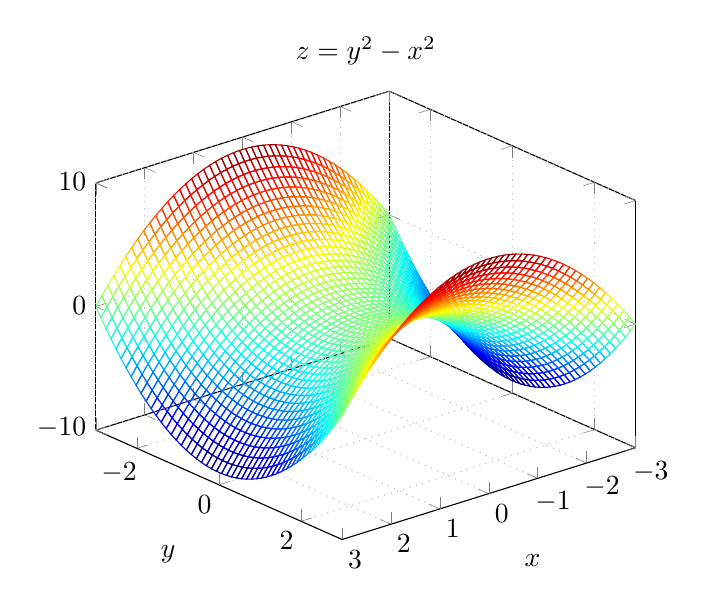
\begin{tikzpicture}
\begin{axis}[
  grid=major,              % draw major gridlines
  major grid style=dotted, % dotted grid lines
  colormap/jet,            % colormap from MATLAB
  samples=50,              % 50 samples in each direction
  view={140}{30},          % configure plot view
  domain=-3:3,             % x varies from -3 to 3
  y domain=-3:3,           % y varies from -3 to 3
  zmin=-10, zmax=10,       % z-axis limits
  xlabel={$x$},            % x-axis label
  xtick={-3,-2,...,3},     % integer-spaced tick marks on the x-axis
  ylabel={$y$},            % y-axis label
  title={$z = y^2 - x^2$},     % plot title
]
\addplot3[mesh] {y^2-x^2}; % make the mesh plot
\end{axis}
\end{tikzpicture}